\subsection*{\textbf{Задание 11.4} Работа с интегралами.}
Вычислите неопределённый и определённый интегралы при $x\in[-9,9]$
функции $y(x) = x^6+3x$.

\begin{figure}[H]
    \renewcommand{\figurename}{Рисунок}
    \centering{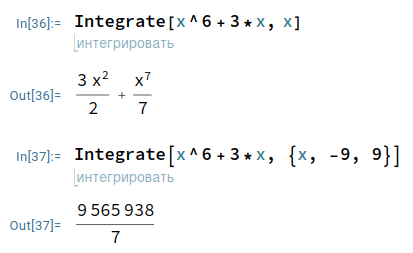
\includegraphics[scale=0.70]{body/img/4.png}}
    \label{fig:image_4}
\end{figure}